\section*{Appendix}

\begin{subappendices}
\section{Details: Materials and Methods}
\subsection{Study procedures and outcome measures}
During their baseline and follow-up visits, all patients were evaluated by research physicians, who collected information on CHF-related symptoms, New York Heart Association (NYHA) class, and performed a physical examination. Information on CHF etiology, left ventricular ejection fraction, cardiovascular risk factors, medical history, and treatment was retrieved primarily from hospital records and was checked in case of ambiguities. History of cardiovascular and other comorbidities was defined as clinical diagnosis thereof reported in the hospital records.

\subsection{Blood sampling and NT-proBNP measurement}
Blood samples were processed and stored at a temperature of -80 degrees C within 2 hours after blood collection. When applicable, samples were transported to the central laboratory (Erasmus MC, Rotterdam, the Netherlands) under controlled conditions (at a temperature of -80 degrees C) until batch analysis was performed. Accordingly, results of the biomarker assays were not available to treating physicians at the time of the outpatient visits and hence did not alter patient care. Plasma NT-proBNP was analyzed using an Electrochemiluminescence immunoassay (Elecsys 2010; Roche Diagnostics, Indianapolis, IN), which measures concentrations ranging from 5 to 35000 ng/L. 

\subsection{Joint Modeling}
We utilized a joint model to estimate the association between longitudinally measured NT-proBNP and clinical outcomes. A joint model combines a linear mixed-effect (LME) model for longitudinally measured data with a Cox regression model for time-to-event data. The use of joint modeling was motivated by the following considerations. In the Bio-SHiFT study, NT-proBNP levels were measured trimonthly until the PE occurred, or until the patient was censored. Thus, naturally, patients who experienced a PE had NT-proBNP measurements available over a shorter time-course than those who did not experience a PE; or in other words, further NT-proBNP measurements could be considered as missing due to occurrence of the PE. However, commonly used methods to model such longitudinal data, for example, linear mixed-effect (LME) models, assume that missing data is non-informative with regard to a patient's health status. In other words, they do not account for the fact that patients with missing NT-proBNP values are more likely to have higher NT-proBNP levels (if hypothetically, we would have been able to observe them). This may lead to bias in the parameter estimates. In addition, a classical time-dependent Cox regression may be used in order to measure the impact of NT-proBNP on the PE. However, due to the aforementioned issue, the time-dependent Cox model may also be biased. To correctly estimate the effects, the parameters of these two types of models are required to be estimated jointly. We did so by applying the joint model.

\subsection{Costs}
Based on the number of scheduled measurements by the personalized and the fixed scheduling approach, we compared the cost estimates from the perspective of Erasmus MC as well as the perspective of society at large for both scheduling approaches. Cost estimates from the perspective of the Erasmus MC included costs of NT-proBNP sampling and measurement, as well as visiting the Cardiology outpatient clinic, at this particular institution~\citep{kanters2017update,hakkaart2015costing}. Cost estimates from the perspective of society at large included average Dutch cost estimates of NT-proBNP sampling and measurement and average Dutch cost estimates of visiting a Cardiology outpatient clinic. Moreover, patients' travel costs and patients' production losses associated with visiting the outpatient clinic were included~\citep{kanters2017update,hakkaart2015costing}.

\section{Supplemental Results}
\subsection{Fixed versus personalized screening schedule: costs}
Costs are depicted in Table~\ref{c6:table:app1}. From the perspective of the Erasmus MC, the costs associated with a visit to the Cardiology outpatient clinic, including blood sampling and NT-proBNP measurement, were €182.1 Thus, since the personalized screening schedule required two visits less than the fixed schedule (Figure~\ref{c6:fig:1}), from the perspective of the Erasmus MC the costs saved by personalized scheduling were on average €364 per patient, over a mean follow-up of 1.76 years (€207 saved per patient per year).

From the perspective of society at large, costs for visiting the outpatient clinic, blood sampling, and NT-proBNP measurement were €106.1 Travel costs and production losses amounted to €6 and €33, respectively. Altogether, costs per visit amounted to €145, with, on average, €290 saved per patient by personalized scheduling versus fixed scheduling, again over a mean follow-up of 1.76 years (€165 saved per patient per year).

In The Netherlands, the prevalence of CHF is estimated at 227,000 patients (\url{www.nivel.nl/node/4309}). In this context, personalized screening could reduce the involved annual costs by approximately €37 million from the perspective of society at large.

\begin{table}
\small
\centering
\caption{\textbf{Cost estimates from the perspective of the Erasmus MC and society at large.} Abbreviations are, CHF: chronic heart failure; NL: The Netherlands; NT-proBNP: N-terminal pro-B-type natriuretic peptide.}
\label{c6:table:app1}
\begin{tabular}{p{6cm}rr}
\toprule
\textbf{Costs} & Erasmus MC (€) & Society at large (€)\\
\midrule
NT-proBNP measurement, per measurement & 19 & 15\\
Visit to outpatient clinic, per visit & 163 & 91\\
Travel costs, per visit	& - & 6\\
Production loss costs, per visit & - & 33\\
Total costs, per visit & 182 & 145\\
\midrule	
Total costs for fixed schedule (median of 9 measurements) & 1638 & 1305\\
Total costs for personalized schedule (median of 7 measurements) & 1274 & 1015\\
Costs saved by personalized scheduling, per patient & 364 & 290\\
Annual costs saved by personalized scheduling (prevalence CHF in NL estimated at 227,000 patients) & - & 37,455,000\\
\bottomrule
\end{tabular}
\end{table}

\begin{figure}
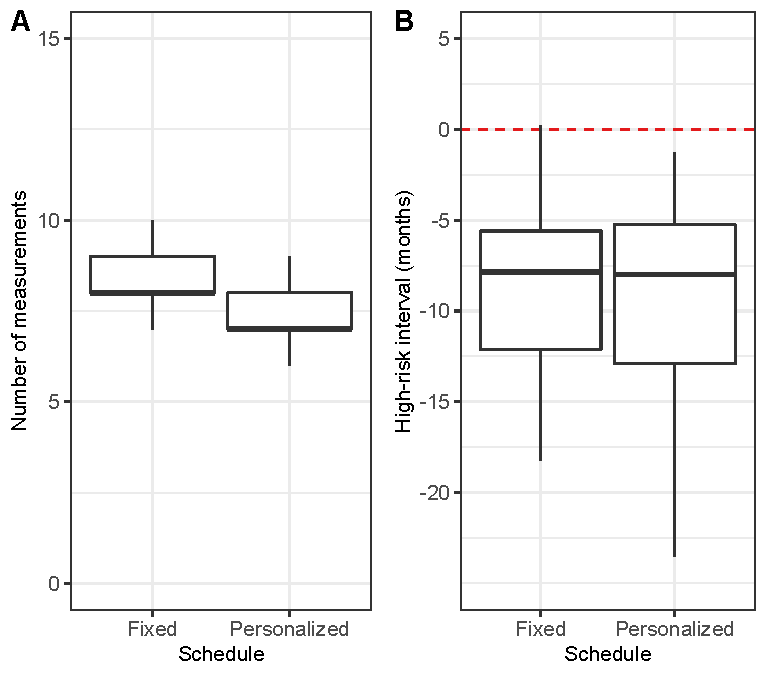
\includegraphics{contents/c6/images/c6_fig_app1.pdf}
\caption{\textbf{Total NT-proBNP measurements and high-risk interval (months) preceding the primary endpoint (PE)} for fixed (quarterly measurements) and personalized schedules. Results are based on a realistic simulation study of 263 test patients. NT-proBNP is measured as per personalized and fixed schedules, until a patient's cumulative-risk of obtaining PE in the subsequent three months is above 5\%. The boxplot for the number of measurements in Panel~A is made using data of all simulated patients. The boxplot for the high-risk interval (the difference between the time at which NT-proBNP measurements are stopped and the true simulated PE time) in Panel~B, is based on only those patients who observe PE. In Panel~B a zero high-risk interval (dashed red line) indicates that no time is available for intervention before occurrence of PE.}
\label{c6:fig:app1}
\end{figure}

\begin{figure}
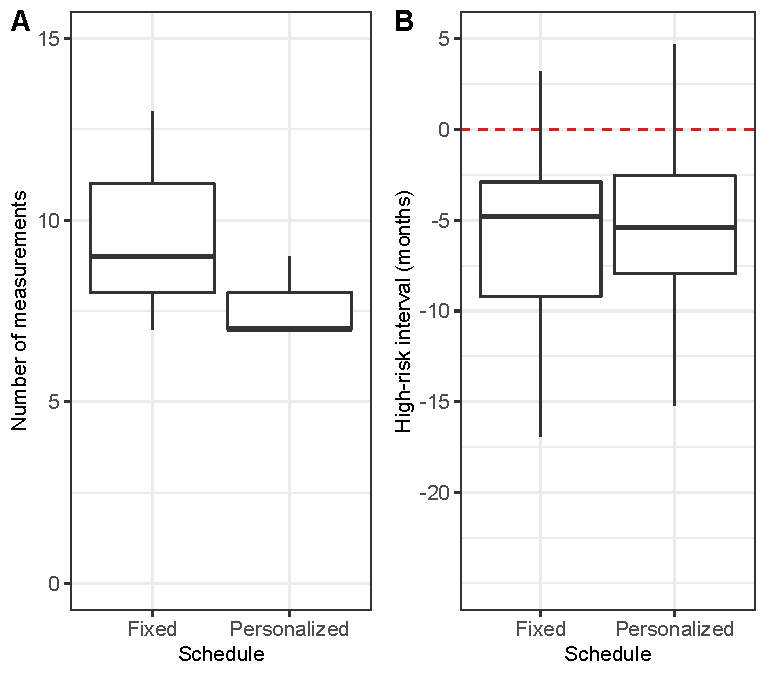
\includegraphics{contents/c6/images/c6_fig_app2.pdf}
\caption{\textbf{Total NT-proBNP measurements and high-risk interval (months) preceding the primary endpoint (PE)} for fixed (quarterly measurements) and personalized schedules. Results are based on a realistic simulation study of 263 test patients. NT-proBNP is measured as per personalized and fixed schedules, until a patient's cumulative-risk of obtaining PE in the subsequent three months is above 10\%. The boxplot for the number of measurements in Panel~A is made using data of all simulated patients. The boxplot for the high-risk interval (the difference between the time at which NT-proBNP measurements are stopped and the true simulated PE time) in Panel~B, is based on only those patients who observe PE. In Panel~B a zero high-risk interval (dashed red line) indicates that no time is available for intervention before occurrence of PE.}
\label{c6:fig:app2}
\end{figure}
\end{subappendices}